\documentclass[12pt,letterpaper,noanswers]{exam}
\usepackage[usenames,dvipsnames,svgnames,table]{xcolor}
\usepackage[margin=0.9in]{geometry}
\renewcommand{\familydefault}{\sfdefault}
\usepackage{multicol}
\usepackage{wrapfig}
\pagestyle{head}
\definecolor{c03}{HTML}{FFDDDD}
\header{AM 22b Class 16}{}{Mar 2: Monte Carlo}
\runningheadrule
\headrule
\usepackage{graphicx} % more modern
\usepackage{amsmath} 
\usepackage{amssymb} 
\usepackage{hyperref}
\usepackage{tcolorbox}

\usepackage[numbered,autolinebreaks,useliterate]{mcode}

\newcommand{\mb}[1]{\underline{#1}}

\begin{document}
 \pdfpageheight 11in 
  \pdfpagewidth 8.5in




% I need to review the torus trajectories...

\begin{itemize}
% \item There is a pre-class assignment (20 minutes of videos + a few WeBWorK exercises) due at 10am this Monday.  It is available on Canvas.
\itemsep0em
    \item Problem set 05 is due on Thursday Mar 11th at 6pm.
  %  \item The Quiz 01 follow up assignment is due on Wednesday Mar 4th at midnight.
    \item The next skill check will be for C16, C17, C18 on Monday Mar 15th.
    \item My Monday OH will occur as scheduled today (3-4pm).
    \item My Wednesday OH will be short this week: 4:30-5pm on Wednesday.  The extra time will be on Thursday from 2:30-3pm this week.
    \item There will be a pre-class assignment for Monday Mar 15th.
\end{itemize}

\hrule
\vspace{0.2cm}

% partial derivatives, gradient
% local linearity, differential, directional deriv
% 2nd order partials + equations with partials

\noindent\textbf{Big picture}

This week we are finishing our introduction to integration for functions of multiple variables.  Today our focus is on numerical approximation of integrals.

\vspace{0.2cm}
\hrule
\vspace{0.2cm}



\noindent\textbf{Skill Check C16 Practice}
\begin{questions}
\question Based on the following code, identify (1) the rectangular box being used to enclose the region of integration, $R$, and (2) the region of integration.

\begin{lstlisting}
fc = @(x,y) x.*y;
npoints = 100000;
xyvals = rand(npoints,2)*2;
indomain = (xyvals(:,1).^2+xyvals(:,2).^2)<4; %set to 1 if in domain; 0 if not
sum(fc(xyvals(:,1),xyvals(:,2)).*indomain)*4/npoints
\end{lstlisting}

\end{questions}


\vspace{0.2cm}
\hrule
\vspace{0.2cm}

\noindent\textbf{Skill Check C16 Solution}

(1) The random numbers are generated in the interval $[0,2]$ (see line 3), so the rectangular box is $0\leq x \leq 2, 0\leq y \leq 2$.

(2) The region of integration comes from line 4: $x^2+y^2 < 4$ (and we have $x,y\geq 0$).  The region is the quarter disk in the first quadrant of the $xy$-plane.

\vspace{0.2cm}
\hrule
\vspace{0.2cm}

\noindent\textbf{Teams}

You will work with this team on the in-class problems today.
\begin{multicols}{2}
1.  students here

\end{multicols}

%\vspace{0.2cm}
\hrule
\vspace{0.2cm}





\noindent\textbf{Quadrature} (not in text)
\begin{tcolorbox}
\begin{itemize}
\itemsep0em
    \item The term \textbf{quadrature} may refer to drawing a square with the same area as a given (planar) shape.  Example: `squaring the circle'.  \emph{Evidently `quadrate' means square}.
    \item \textbf{Quadrature} is also the term used to refer to finding an integral numerically.
    \item A \textbf{quadrature rule} determined by a set of nodes, $x_k \in [a,b]$, and a set of coefficients, $a_k$: $\displaystyle Q(f) = \sum\limits_{k=1}^n a_k f(x_k)$.  The \textbf{left Riemann sum} for approximating an integral, $\displaystyle Q(f) = \sum\limits_{k=1}^n \frac{1}{n}f(a + (k-1)h)$ with $h = \frac{b-a}{n}$,  is an example of a quadrature rule.  The \textbf{right Riemann sum}, $\displaystyle Q(f) = \sum\limits_{k=1}^n \frac{1}{n}f(a + h)$ with $h = \frac{b-a}{n}$, is another example.
    \item A quadrature rule for approximating an integral of a function $f$ has an associated \textbf{error}.  The error will depend on the properties of the function (specifically on its derivatives).
\end{itemize}
\end{tcolorbox}

\noindent\textbf{Example} (trapezoidal rule; over 2000 years old).

Consider $\int_0^1 f(x)\ dx$.  Write down a quadrature rule for approximating this integral.  Use the midpoint/trapezoidal rule, and use four even subintervals.
\vspace{1in}


\noindent\textbf{Example} (left Riemann sum: 2d)

\begin{multicols}{2}

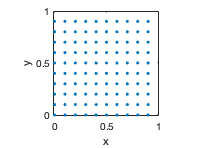
\includegraphics{img/C15domainright.png}

\begin{lstlisting}
fc = @(x,y) x.^2 + y.^2;
h = 1/10;
valleft = 0;
for k1 = 0:h:1-h
    for k2 = 0:h:1-h
        valleft = valleft + fc(k1,k2)*h^2;
    end
end
\end{lstlisting}
\end{multicols}

Based on the code above, identify the function of integration.  Make an informed guess for the region of integration.


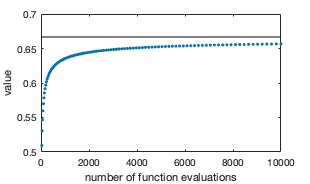
\includegraphics[width=0.45\textwidth]{img/C15leftdet.png}
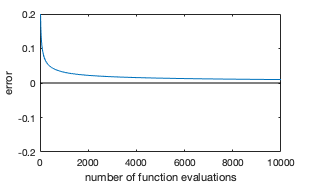
\includegraphics[width=0.45\textwidth]{img/C15leftdeterror.png}

The plot on the left is showing the value of the quadrature (and the actual value of the integral) as the number of grid boxes (and thus the number of function evaluations) increases.

The plot on the right is showing the error: the difference between the actual value of the integral and the approximation via this quadrature rule.

% \vspace{0.2cm}
% \hrule
% \vspace{0.2cm}

% \noindent\textbf{Monte Carlo integration} (not in text)
% \begin{tcolorbox}
% \begin{itemize}
% \itemsep0em
%     \item \textbf{Monte Carlo integration} is an even weight quadrature where the set of nodes is chosen randomly (usually using a uniform distribution over the unit box).
%     \item The \textbf{unit box} in $\mathbb{R}^n$ is $[0,1]\times [0,1] ...\times [0,1] = [0,1]^n$.  In $\mathbb{R}$ this is the unit interval while in $\mathbb{R}^2$ this is the unit square.
% \end{itemize}
% \end{tcolorbox}

% \noindent\textbf{Example} (Monte Carlo quadrature points)

% \begin{multicols}{2}
% 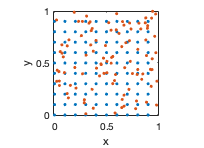
\includegraphics{img/C15domain.png}

% \begin{lstlisting}
% [xval,yval] = meshgrid(0:0.1:0.9,0:0.1:0.9);
% plot(xval(:),yval(:),'.')
% hold on
% xyrand = rand(100,2);
% plot(xyrand(:,1),xyrand(:,2),'.')
% axis equal
% axis([-0.01 1 -0.01 1])
% xlabel('x'); ylabel('y')
% \end{lstlisting}
% \end{multicols}

% The quadrature points are shown in red for the Monte Carlo integration.  Identify the line of code associated with generating those points.

% \vspace{0.1in}

% \noindent\textbf{Example} (Monte Carlo integration)

% \begin{multicols}{2}
% \begin{lstlisting}
% % with a loop
% fc = @(x,y) x.^2 + y.^2;
% sumcount = 0;
% npoints = 10000;
% xyvals = rand(npoints,2);
% for numrum = 1:npoints
%     sumcount = sumcount + fc(xyvals(numrum,1),xyvals(numrum,2));
% end
% integral = sumcount/npoints;
% \end{lstlisting}
% \columnbreak
% \begin{lstlisting}
% % with a vector
% fc = @(x,y) x.^2 + y.^2;
% npoints = 10000;
% xyvals = rand(npoints,2);
% integral = sum(fc(xyvals(:,1),xyvals(:,2)))/npoints;
% \end{lstlisting}
% \end{multicols}

% 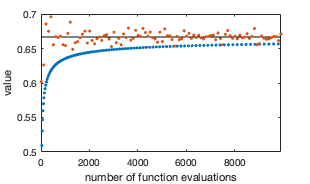
\includegraphics[width=0.45\textwidth]{img/C15MC.png}
% 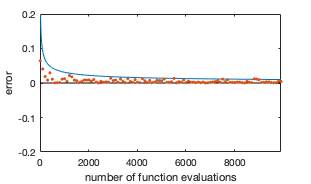
\includegraphics[width=0.45\textwidth]{img/C15MCerror.png}

% \vspace{0.2cm}
% \hrule
% \vspace{0.2cm}

% \noindent\textbf{Monte Carlo integration: other domains} (not in text)
% \begin{tcolorbox}
% To use \textbf{Monte Carlo integration} over a region that is not the unit box:
% \begin{itemize}
% \itemsep0em
%     \item Create a rectangular box that encloses the region.  
%     \item Define the function piecewise: it will be $0$ everywhere that is outside the region but inside the box.  It will be $f(\underline{x})$ inside the region.
%     \item Use Monte Carlo integration on the rectangular box.
% \end{itemize}
% \end{tcolorbox}

%     \noindent\textbf{Example} (A non-unit interval in Matlab)
    
%     \texttt{5*rand(1)} generates a random number uniformly spaced between $0$ and $5$.  \texttt{4*rand(1)+1} generates a random number uniformly spaced between $1$ and $5$.
    
%     Write an expression to generate a pair of random numbers with one between $-1$ and $1$ and the second between $2$ and $4$.
%     \vspace{1in}
    
    

% \noindent\textbf{Example: Approximating $\pi$}

% Let $f(x,y) = 4$.  Let $R$ be the region in the first quadrant where $x^2+y^2\leq 1$.  $\int_R f(x,y) dA = \int_0^{\pi/2}\int_0^1 4r\ dr\ d\theta = \pi$.

% Approximate this numerically to find an estimate for $\pi$.
% \begin{lstlisting}   
% npoints = 100000;
% xyvals = rand(npoints,2);
% indomain = (xyvals(:,1).^2+xyvals(:,2).^2)<1; %set to 1 if in domain; 0 if not
% sum(4*indomain)/npoints
% \end{lstlisting}

% 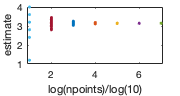
\includegraphics{img/C15Mpi.png}
% 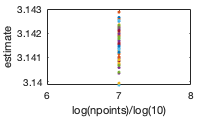
\includegraphics{img/C15MCpi7.png}
% \vspace{0.1cm}

% \noindent\textbf{Example: circular region}

% Approximate the integral of a function that is not uniform: let $f(x,y) = xy$.  Let $R$ be the region in the first quadrant where $x^2+y^2\leq 1$.

% \begin{lstlisting}
% fc = @(x,y) x.*y;
% npoints = 100000;
% xyvals = rand(npoints,2);
% indomain = (xyvals(:,1).^2+xyvals(:,2).^2)<1; %set to 1 if in domain; 0 if not
% sum(fc(xyvals(:,1),xyvals(:,2)).*indomain)/npoints
% %% Analytically:
% int(int(fc(x,y),x,0,sqrt(1-y.^2)),y,[0,1])
% \end{lstlisting}


\vspace{0.2cm}
\hrule
\vspace{0.2cm}



\noindent\textbf{Monte Carlo integration} (not in text)
\begin{tcolorbox}
\begin{itemize}
\itemsep0em
\item For many functions, an integral cannot be computed analytically: numerical approximation is the main option in that case.
    \item \textbf{Monte Carlo integration} is an even weight quadrature where the set of nodes is chosen randomly (usually using a uniform distribution over the unit box).
    \item The \textbf{unit box} in $\mathbb{R}^n$ is $[0,1]\times [0,1] ...\times [0,1] = [0,1]^n$.  In $\mathbb{R}$ this is the unit interval while in $\mathbb{R}^2$ this is the unit square.
\end{itemize}
\end{tcolorbox}

\noindent\textbf{Example} (Monte Carlo quadrature points)

\begin{multicols}{2}
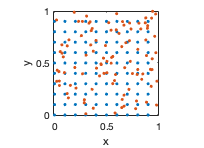
\includegraphics{img/C15domain.png}

\begin{lstlisting}
[xval,yval] = meshgrid(0:0.1:0.9,0:0.1:0.9);
plot(xval(:),yval(:),'.')
hold on
xyrand = rand(100,2);
plot(xyrand(:,1),xyrand(:,2),'.')
axis equal
axis([-0.01 1 -0.01 1])
xlabel('x'); ylabel('y')
\end{lstlisting}
\end{multicols}

The quadrature points are shown in red for the Monte Carlo integration.  Identify the line of code associated with generating those points.

\vspace{1in}

\noindent\textbf{Example} (Monte Carlo integration)

\begin{multicols}{2}
\begin{lstlisting}
% with a loop
fc = @(x,y) x.^2 + y.^2;
sumcount = 0;
npoints = 10000;
xyvals = rand(npoints,2);
for numrum = 1:npoints
    sumcount = sumcount + fc(xyvals(numrum,1),xyvals(numrum,2));
end
integral = sumcount/npoints;
\end{lstlisting}
\columnbreak
\begin{lstlisting}
% with a vector
fc = @(x,y) x.^2 + y.^2;
npoints = 10000;
xyvals = rand(npoints,2);
integral = sum(fc(xyvals(:,1),xyvals(:,2)))/npoints;
\end{lstlisting}
\end{multicols}

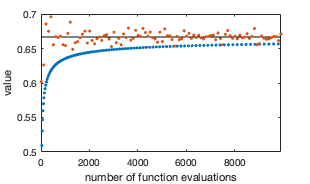
\includegraphics[width=0.45\textwidth]{img/C15MC.png}
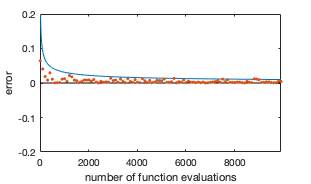
\includegraphics[width=0.45\textwidth]{img/C15MCerror.png}

\vspace{0.2cm}
\hrule
\vspace{0.2cm}

\noindent\textbf{Monte Carlo integration: other domains} (not in text)
\begin{tcolorbox}
To use \textbf{Monte Carlo integration} over a region, $R$ that is not the unit box:
\begin{itemize}
\itemsep0em
    \item Create a rectangular box that encloses the region, $R$ and has area $A_{box}$. 
    \item Define the function piecewise: it will be $0$ everywhere that is outside $R$.  It will be $f(\underline{x})$ in the region $R$.
    \item To use Monte Carlo integration on the rectangular box, generate $N$ random points within the box.  Sum the function evaluated at each point.  Multiply by the area of the box divided by the number of points: $A_{box}/N$ (this is the average area associated with each function evaluation).
    \begin{lstlisting}
% Example
fc = @(x,y) x.^2 + y.^2;
npoints = 10000;
xyvals = rand(npoints,2);
xyvals(:,1) = xyvals(:,1)*5;
xyvals(:,2) = xyvals(:,2)*7;
integral = sum(fc(xyvals(:,1),xyvals(:,2)))*5*7/npoints;
\end{lstlisting}
\end{itemize}

\textbf{Pseudocode} is a description of the steps in a computer program, where the instructions may be written in human language, rather than in the syntax of a programming language.
\end{tcolorbox}

    \noindent\textbf{Example} (A non-unit interval in Matlab)
    
    \texttt{5*rand(1)} generates a random number uniformly spaced between $0$ and $5$.  \texttt{4*rand(1)+1} generates a random number uniformly spaced between $1$ and $5$.
    
    Write pseudocode to generate a pair of random numbers with one between $-1$ and $1$ and the second between $2$ and $4$.
    \vspace{1in}
    
    \eject

\noindent\textbf{Example: Approximating $\pi$}

Let $f(x,y) = 4$.  Let $R$ be the region in the first quadrant where $x^2+y^2\leq 1$.  $\int_R f(x,y) dA = \int_0^{\pi/2}\int_0^1 4r\ dr\ d\theta = \pi$.

Approximate this numerically to find an estimate for $\pi$.
\begin{lstlisting}   
npoints = 100000;
xyvals = rand(npoints,2);
indomain = (xyvals(:,1).^2+xyvals(:,2).^2)<1; %set to 1 if in domain; 0 if not
sum(4*indomain)/npoints
\end{lstlisting}

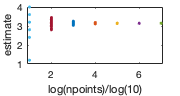
\includegraphics{img/C15Mpi.png}
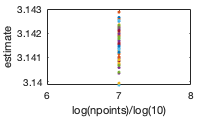
\includegraphics{img/C15MCpi7.png}
\vspace{0.1cm}

\noindent\textbf{Example: circular region}

Approximate the integral of a function that is not uniform: let $f(x,y) = xy$.  Let $R$ be the region in the first quadrant where $x^2+y^2\leq 1$.

\begin{lstlisting}
fc = @(x,y) x.*y;
npoints = 100000;
xyvals = rand(npoints,2);
indomain = (xyvals(:,1).^2+xyvals(:,2).^2)<1; %set to 1 if in domain; 0 if not
sum(fc(xyvals(:,1),xyvals(:,2)).*indomain)/npoints
%% Analytically:
int(int(fc(x,y),x,0,sqrt(1-y.^2)),y,[0,1])
\end{lstlisting}

\vspace{1in}

\noindent\textbf{Example}

%\begin{tabular}{p{12cm} c }
Provide pseudocode for using Monte-Carlo integration to approximate the area, $\int_R dA$, where $R$ is the crescent shape shown. %&

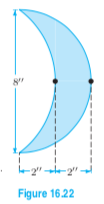
\includegraphics[scale=0.65]{img/C16crescent.png}
%\end{tabular}


\end{document}